%-------------------------------------------------------------------------------
%-------------------------------------------------------------------------------

This analysis studied the use of a multiclass BDT that differentiates between VBF Higgs, ggF Higgs, and SM WW backgrounds for the final statistical fit. This BDT showed success at differentiating VBF signal from WW backgrounds but found very little discrimination with ggF. Using the ABCD method and targeted ggF control regions and discriminants showed better overall signal significance in the final statistical fit. While this BDT was not used, its optimization informed the choice of input variables and settings for the one-dimensional BDTs that were ultimately chosen. 

The boosted decision tree training algorithm used in the multiclass BDT training used the TMVA gradient boosting algorithm to discriminate between three classes of events. A collection of cuts is designed to classify events as $WW$-like, ggF-like, or VBF-like. After the initial tree is built, another tree is grown to better separate the misclassified events. This proceeds iteratively until there is a collection of a specified number of trees (``boosting''). A weighted average is taken from all these trees to form a BDT output discriminant with values ranging from 0 to 1.

The multiclass BDT is trained using $e\mu+\mu e$ events after the VBF pre-selection and the signal regions cuts including that on $n_{jets}$, $b$-veto, OLV, CJV, $M_{jj}$, $\Delta Y_{jj}$, and a cut on the $\Ztt$ BDT (described in Appendix B). The phase space in which we train the BDT is exactly the same as the one where we apply it. The training includes the $WW$ background, $ggF$ background and the VBF signal, each defined in the main text. The MC statistics used in the training are half those available after all signal region cuts. This corresponds to $\approx$ 500,000 $WW$ events, $\approx$ 20,000 $ggF$, and $\approx$100,000 VBF events.

The TMVA BDTG interface is used to train and test the multiclass BDT. The optimal parameters were found through a scan of reasonable values and the final set is summarized in Table~\ref{tab:multiBDTparameters}.

\begin{table}[h!]
\centering
\begin{tabular}{|l|c|c|}
\hline
Parameter                                    & Value    & Range     \\
\hline
Boosting algorithm                           & Gradient & --        \\
Maximum tree depth                           &  5       & [3,10,22,30]    \\
Number ofapter{$Z+$jets BDT}
Number of trees                              &  1000    & [200,1000,10000] \\
Minimum number of events requires per mode   &  5\%     & [5\%]\\
Number of cuts                               &  10       & [5,7,10,12]  \\
\hline
\end{tabular}
\caption{Tested and optimal parameters for multiclassification BDT.}
\label{tab:multiBDTparameters}
\end{table}

For this BDT, variables were carefully chosen to optimize differences between each of the three classifications. Over 25 potentially useful variables were tested in the multiclass BDT and the most impactful of these were chosen. Training variables for the optimal analysis include $M_{l1j1}$, $M_{l1j0}$, $M_{l0j1}$, $M_{l0j0}$, $\sum \eta_\ell^{\mathrm{centrality}}$, $\Delta \phi_{jj}$, $p_T^{j0}$, $p_T^{j1}$, $p_T^{j2}$, $\eta^{j0}$, $\eta^{j1}$, $\eta^{l0}$, $\eta^{l1}$, $p_T^{l0}$, $p_T^{l1}$, $p_T^{\text{tot}}$, $\Delta \eta_{jj}$, $\sum \eta_{jj}$, $m_T$, $m_{ll}$, $\Delta \phi_{\ell\ell}$, $\Delta Y_{\ell\ell}$, $\sum M_{lj}$, and $\Delta Y_{jj}$. Figure~\ref{fig:multiclassBDTinput} and~\ref{fig:multiclasscorrSB} show the input distributions of each variable used to train the multiclass BDT and the correlations between them.

BDT input variables are ranked by importance through a TMVA algorithm. The algorithm determines how often the each variable is used to split decision tree nodes and then weights each split by the squared separation gain achieved and by the number of events in that node~\ref{TMVA}. Ranking results are displayed in order of variable importance in Table~\ref{tab:rankingmulti}.

\begin{table}[h!]
\centering
\begin{tabular}{|l|c|c|}
\hline
Rank &	Variable  & BDT Importance \\
\hline
1 &  $\Delta \phi_{ll}$ & 7.2    \\
2 &  $\Delta \phi_{jj}$ &  7.2\\
3 &  $\Delta Y_{jj}$   & 7.1    \\
4 &  $\sum\eta_\ell^{\mathrm{centrality}}$ & 6.8   \\
5 &  $\eta^{j1}$ &  6.3  \\
6 &  $m_T$     &  6.2  \\
7 &  $\eta^{j0}$ &  6.2  \\
8 &  $\Delta Y_{\ell\ell}$   & 5.0   \\
9 &  $p_T^{j0}$  & 4.9   \\
10  & $p_T^{j1}$ & 4.7   \\
11  & $\sum M_{lj}$& 4.4   \\
12  & $p_T^{tot}$ & 4.2   \\
13  & $M_{l0j1}$& 4.1   \\
14  & $M_{l1j0}$& 3.9   \\
15  & $m_{\ell\ell}$   & 3.8   \\
16  & $p_T^{l1}$  & 3.8   \\
17  & $M_{l1j1}$& 3.7   \\
18  & $p_T^{j2}$  & 3.7   \\
19  & $M_{l0j0}$& 3.6   \\
20  & $p_T^{l0}$  & 3.3   \\ 
\hline
\end{tabular}
\caption{Input variables to multiclass BDT ranked in order or importance}
\label{tab:rankingmulti}
\end{table}

\begin{figure}[!htbp]
    \centering
    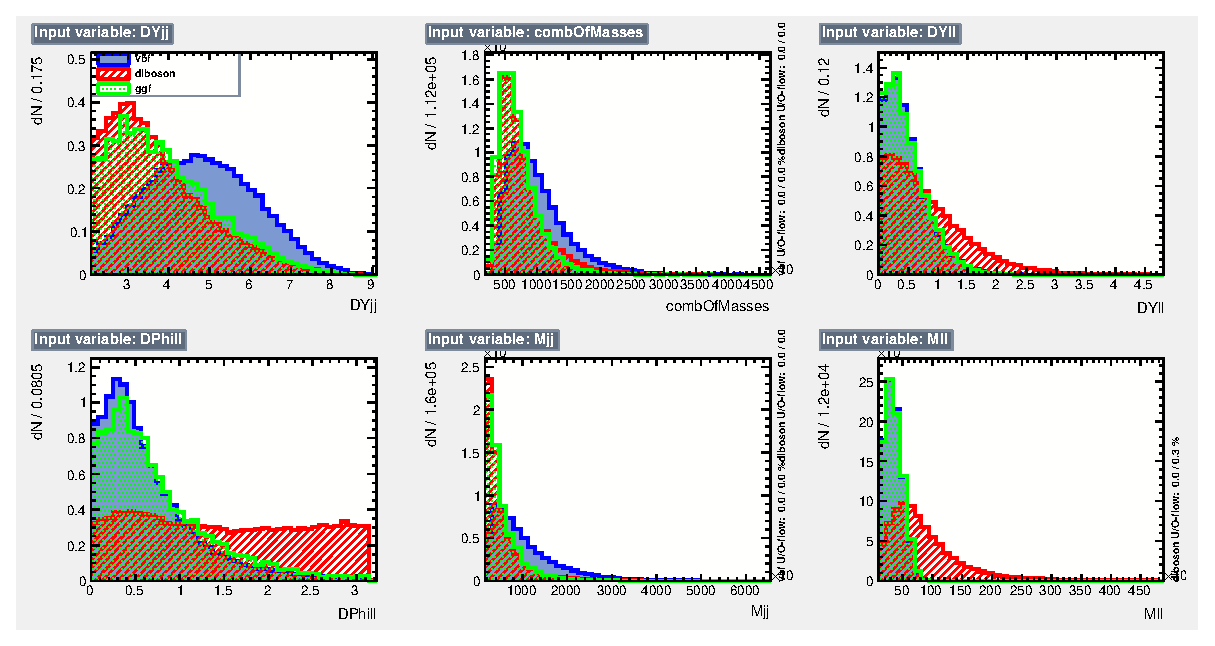
\includegraphics[width=0.45\linewidth]{Pictures/finalBDT_def/variables_id_c1.eps} \quad
    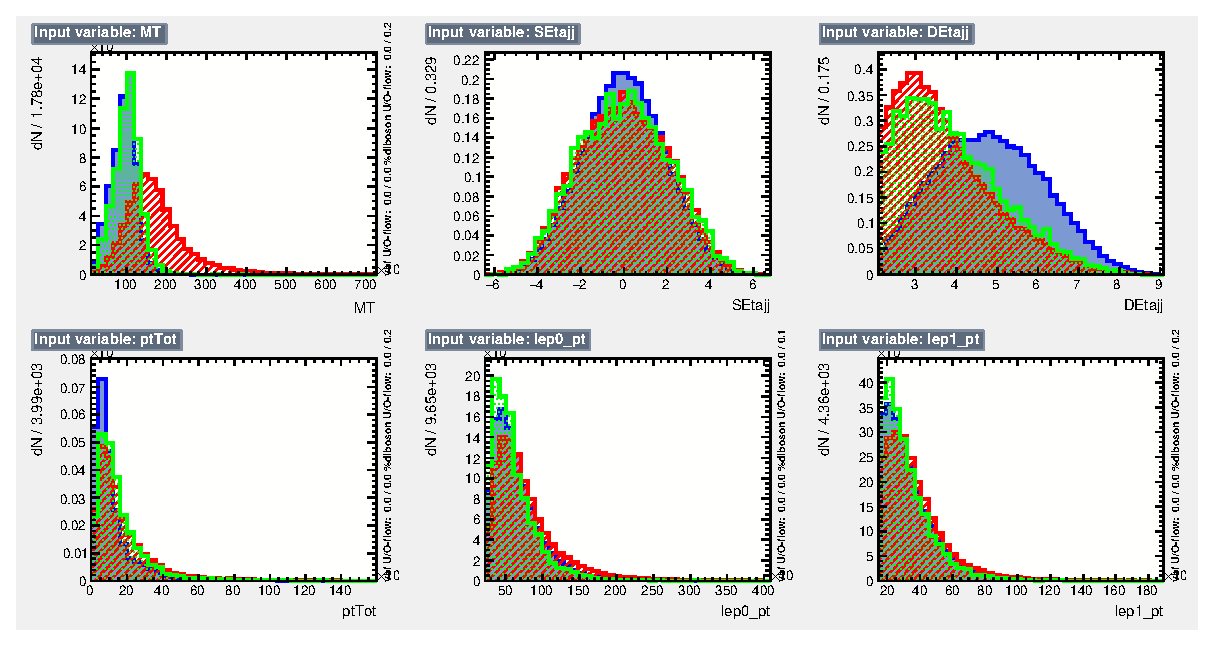
\includegraphics[width=0.45\linewidth]{Pictures/finalBDT_def/variables_id_c2.eps} 
    \medskip
    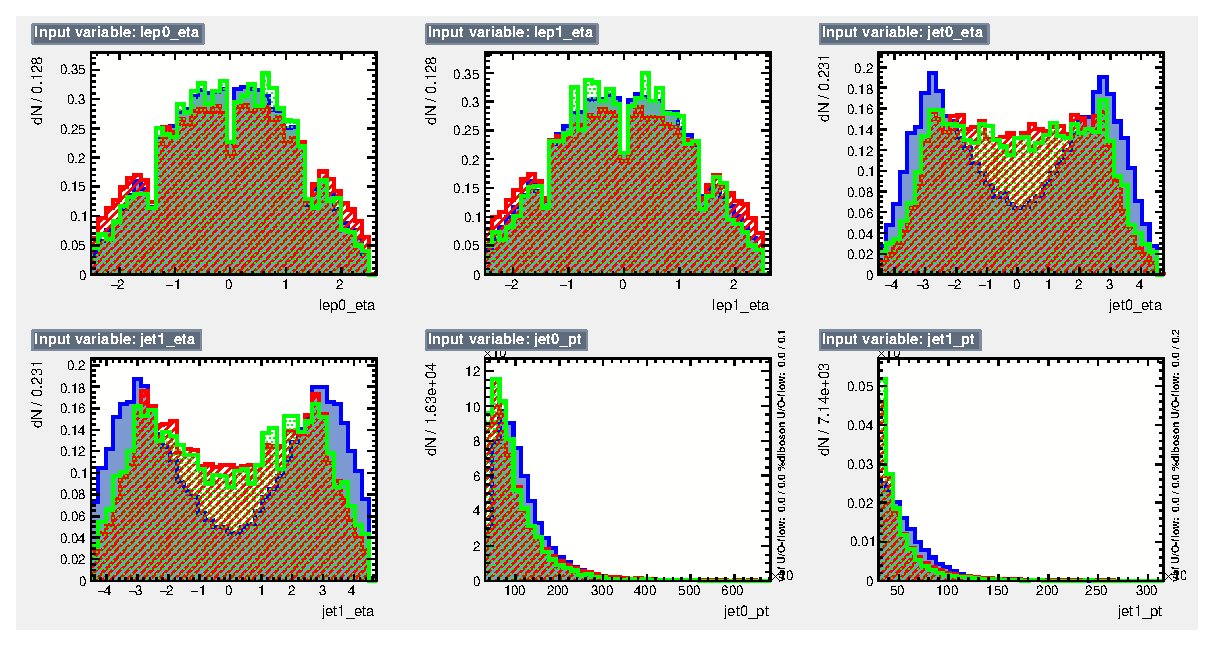
\includegraphics[width=0.45\linewidth]{Pictures/finalBDT_def/variables_id_c3.eps} \quad
    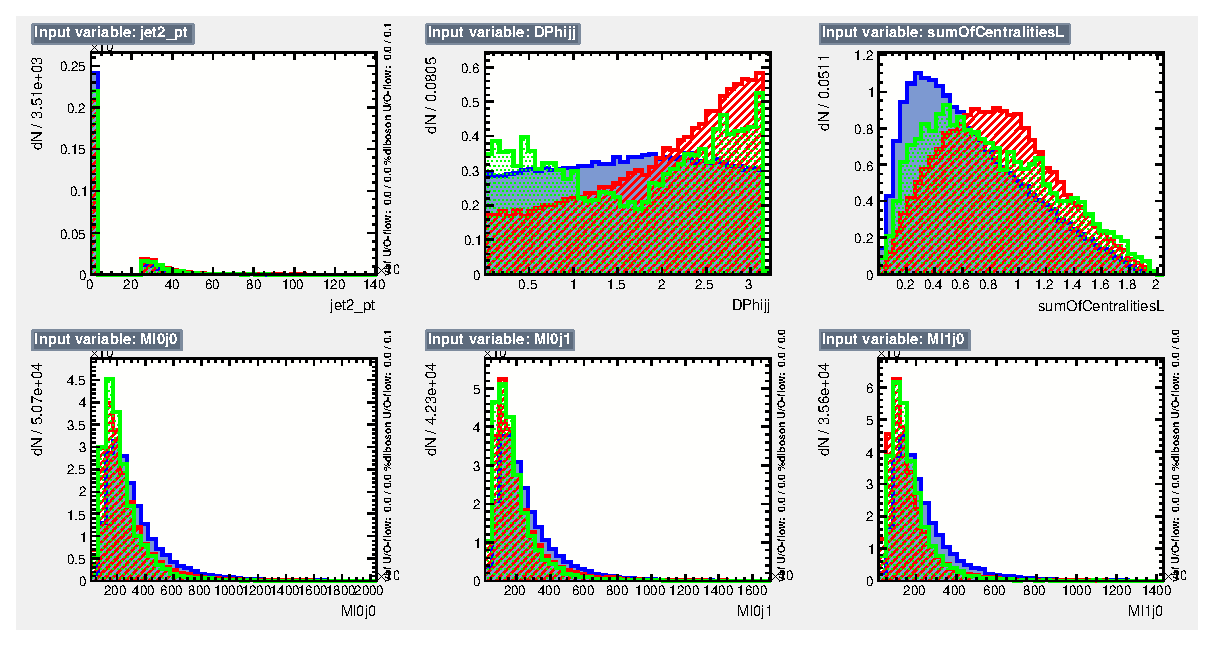
\includegraphics[width=0.45\linewidth]{Pictures/finalBDT_def/variables_id_c4.eps} 
    \medskip
    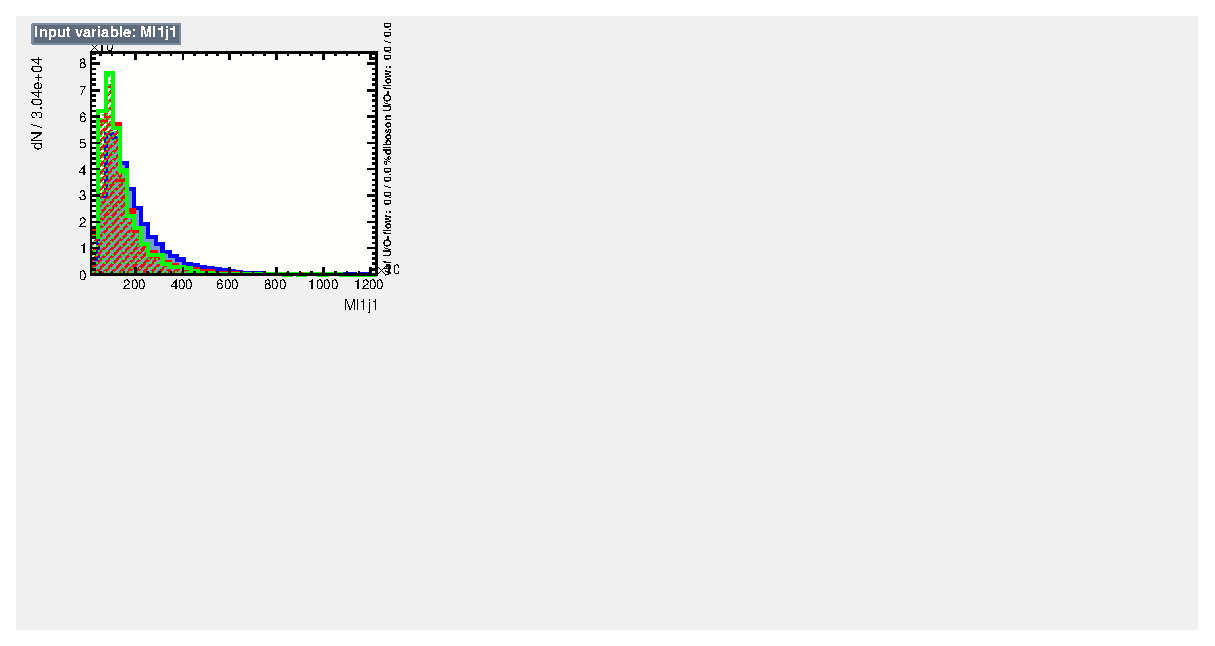
\includegraphics[width=0.45\linewidth]{Pictures/finalBDT_def/variables_id_c5.eps}
    \caption{Distributions of input variables to the multiclass BDT. Samples are normalized to even contributions from each event type.}
    \label{fig:multiclassBDTinput}
\end{figure}
%
\begin{figure}[!htbp]
\centering
  \includegraphics[width=.33\linewidth]{Pictures/finalBDT_def/CorrelationMatrixvbf.eps}
  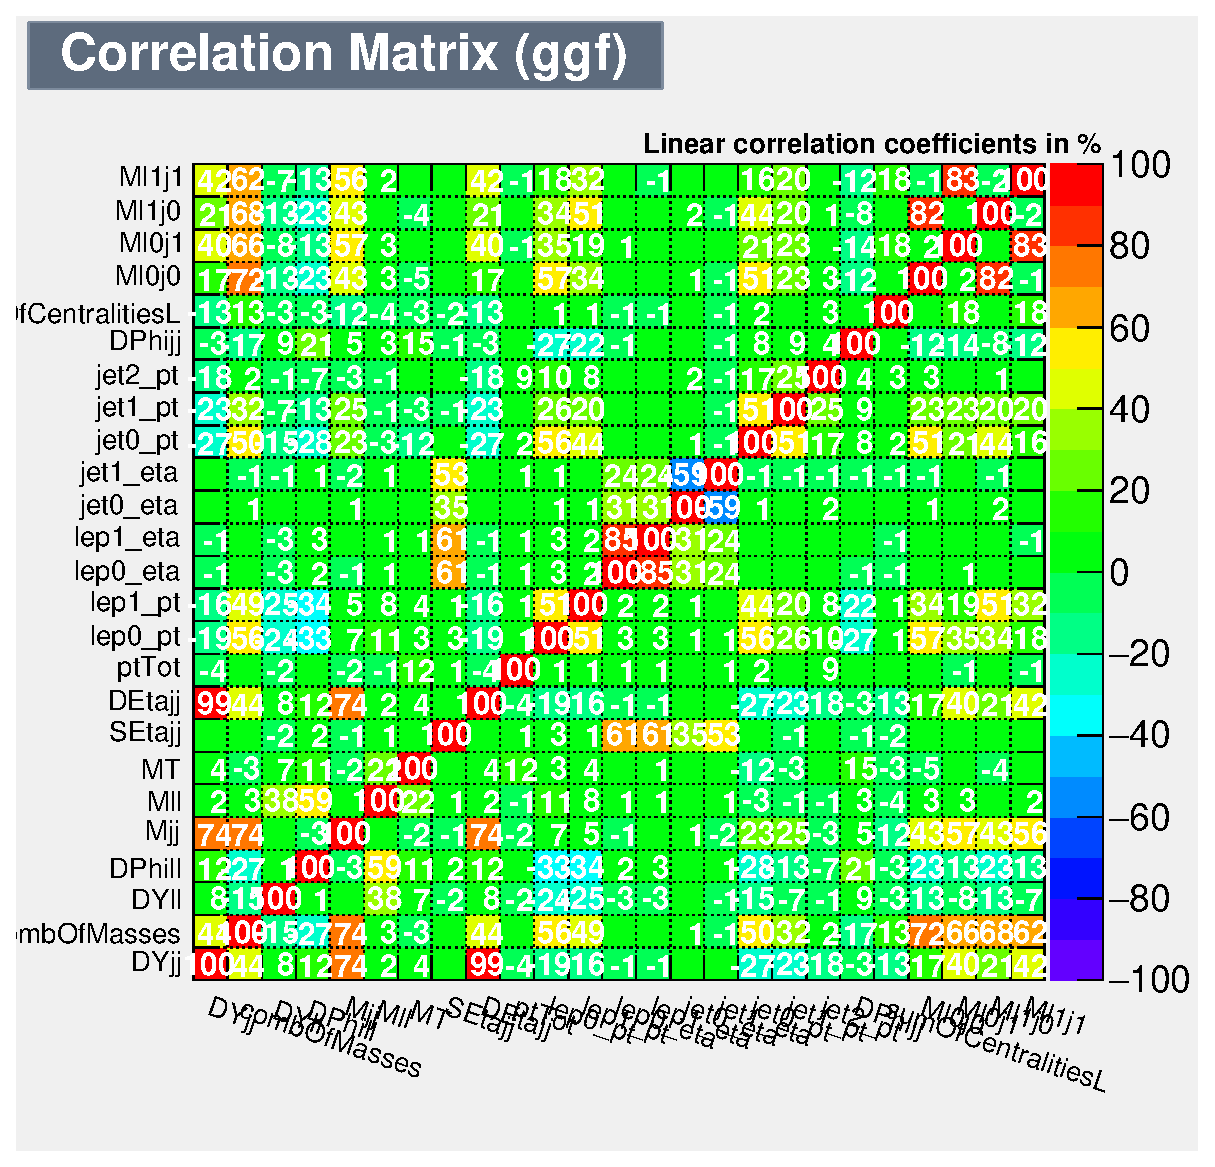
\includegraphics[width=.33\linewidth]{Pictures/finalBDT_def/CorrelationMatrixggf.eps}
  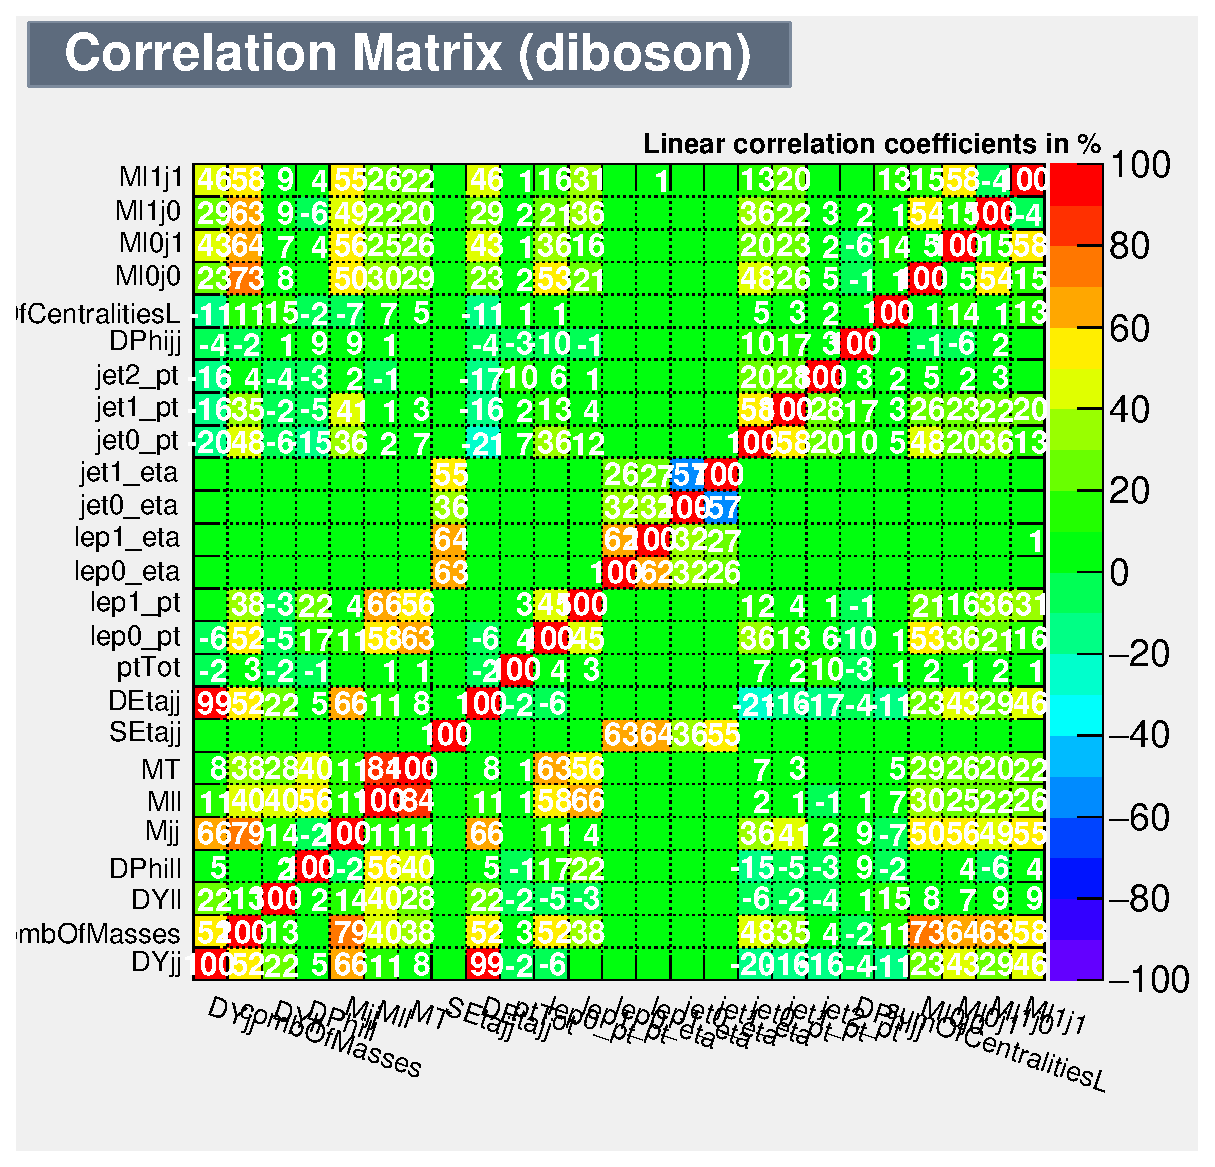
\includegraphics[width=.33\linewidth]{Pictures/finalBDT_def/CorrelationMatrixdiboson.eps}
\caption{Correlations of input variables to the multiclass BDT. Plots show correlations for VBF (left), ggF (center) and WW events (right).}
\label{fig:multiclasscorrSB}
\end{figure}

In order to quantify the discrimination, we use the integrated-ROC calculated through TMVA for normalized samples and find an optimal value of 0.939 (VBF), 0.804 (ggF), and 0.947 (WW). Comparisons between the test and training show that the BDT is un-biased--differences between testing and training samples would imply overtraining, or the BDT using to many parameters on too few events. Visually, one can see that the testing and trainings samples are quite similar. Figure~\ref{fig:multiclassBDTresult} shows BDT output results applied to normalized samples of VBF, ggF, and WW. Figure~\ref{fig:multiclassBDTresult2} shows all backgrounds as well as the three trained samples with all event weights applied in order to understand how the entire dataset distributes with the BDT output. Since our BDT is trained in three dimensions, Figure~\ref{fig:multiclassBDTresult2} shows projections onto each axis. Figure~\ref{fig:multiclass3D} similarly shows results in three dimensions to understand correlations between the sample outputs.

\begin{figure}[!htbp]
\centering
  \centering
  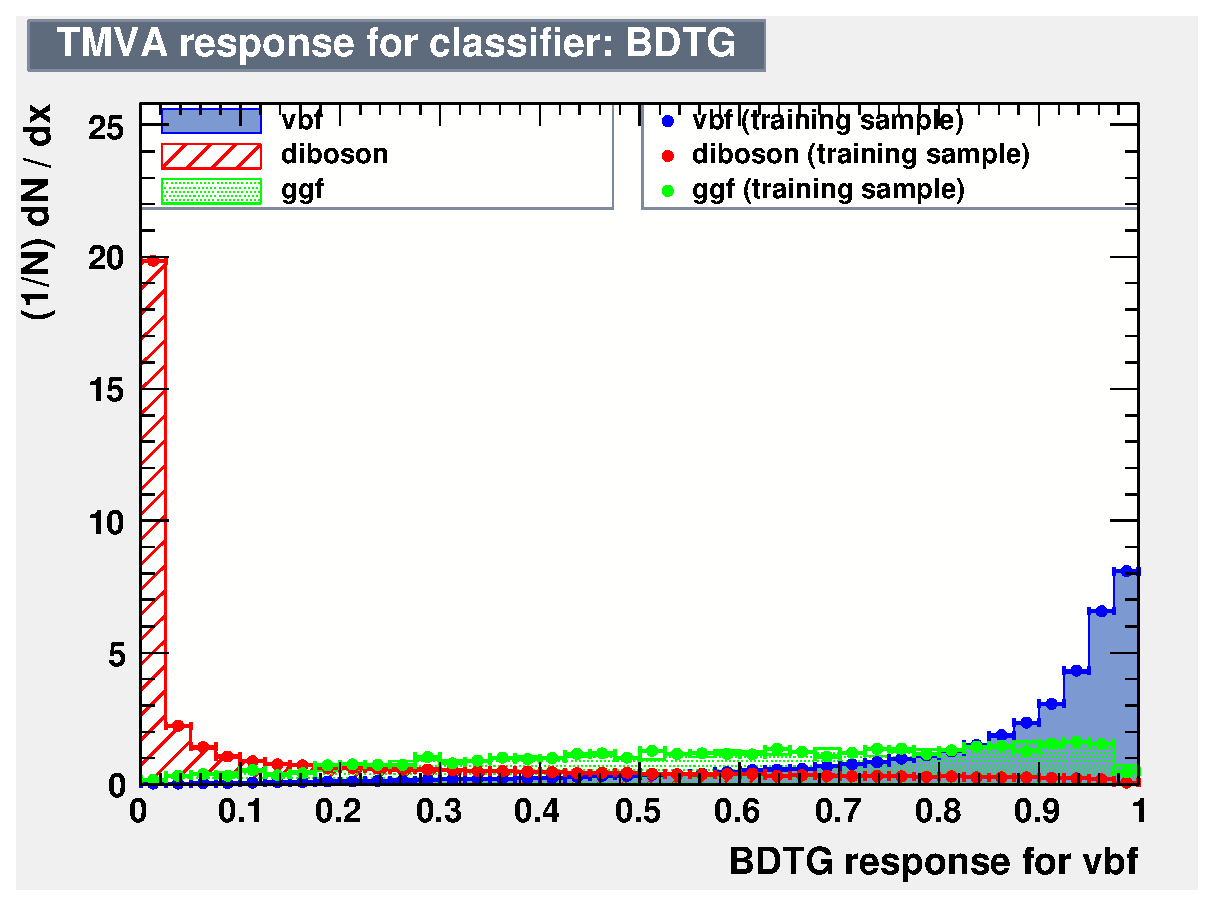
\includegraphics[width=.3\linewidth]{Pictures/finalBDT_def/overtrain_vbf_BDTG.eps} \quad
  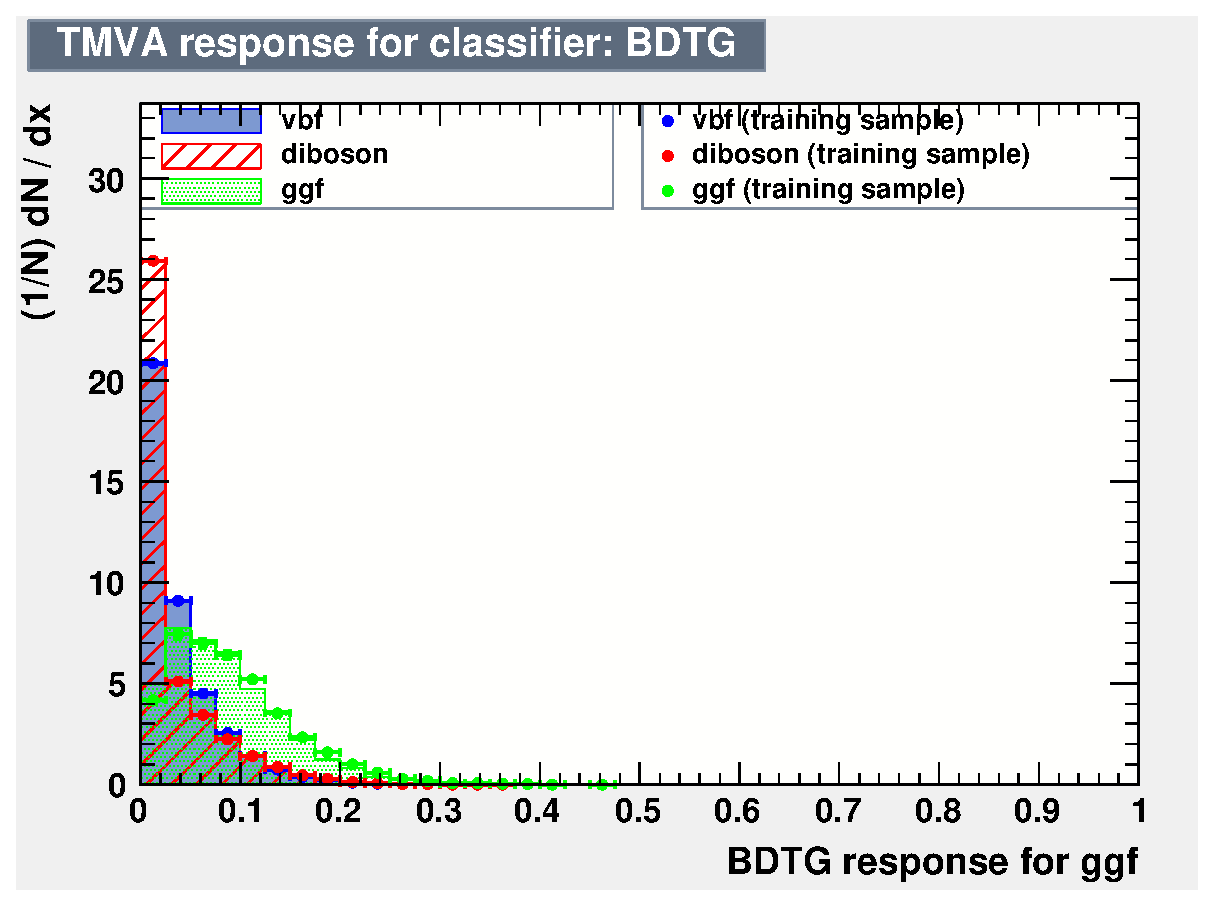
\includegraphics[width=.3\linewidth]{Pictures/finalBDT_def/overtrain_ggf_BDTG.eps} \quad
  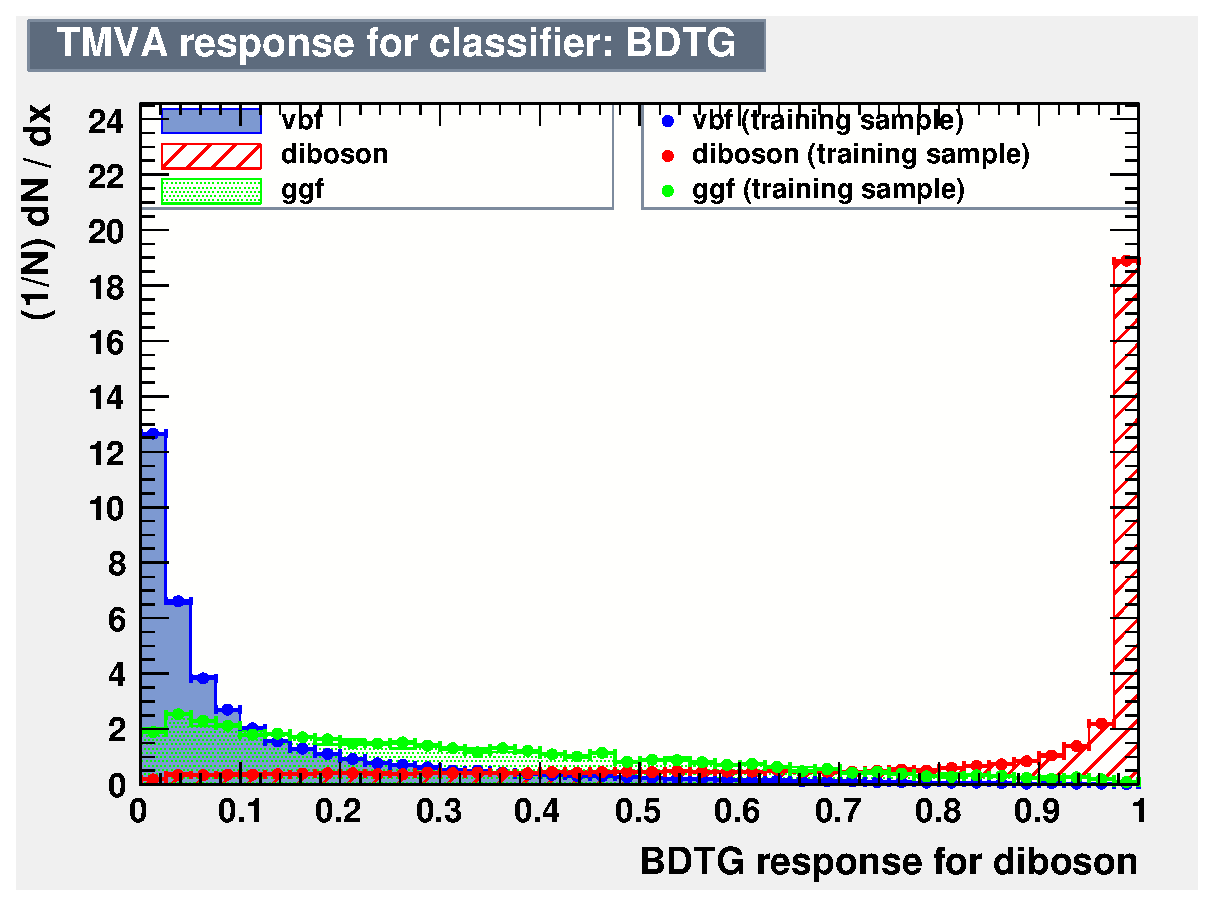
\includegraphics[width=.3\linewidth]{Pictures/finalBDT_def/overtrain_diboson_BDTG.eps}
\caption{Normalized samples of VBF, ggF, and WW plotted over BDT output distribution, overlaid testing and training samples shown.}
\label{fig:multiclassBDTresult}
\end{figure}
\begin{figure}[!htbp]
\centering
  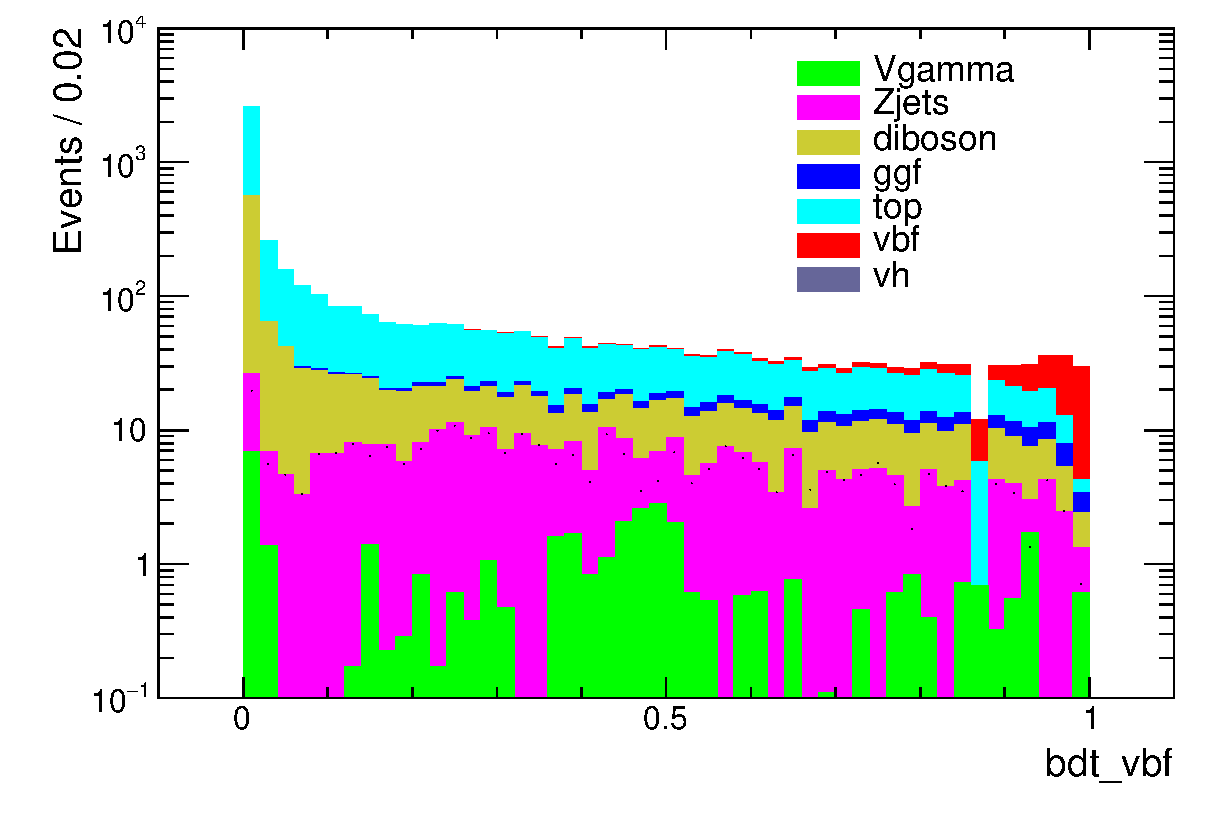
\includegraphics[width=.3\linewidth]{Pictures/finalBDT_def/weightedmulticlassvbf.eps} \quad
  \includegraphics[width=.3\linewidth]{Pictures/finalBDT_def/weightedmulticlassggf.eps} \quad
  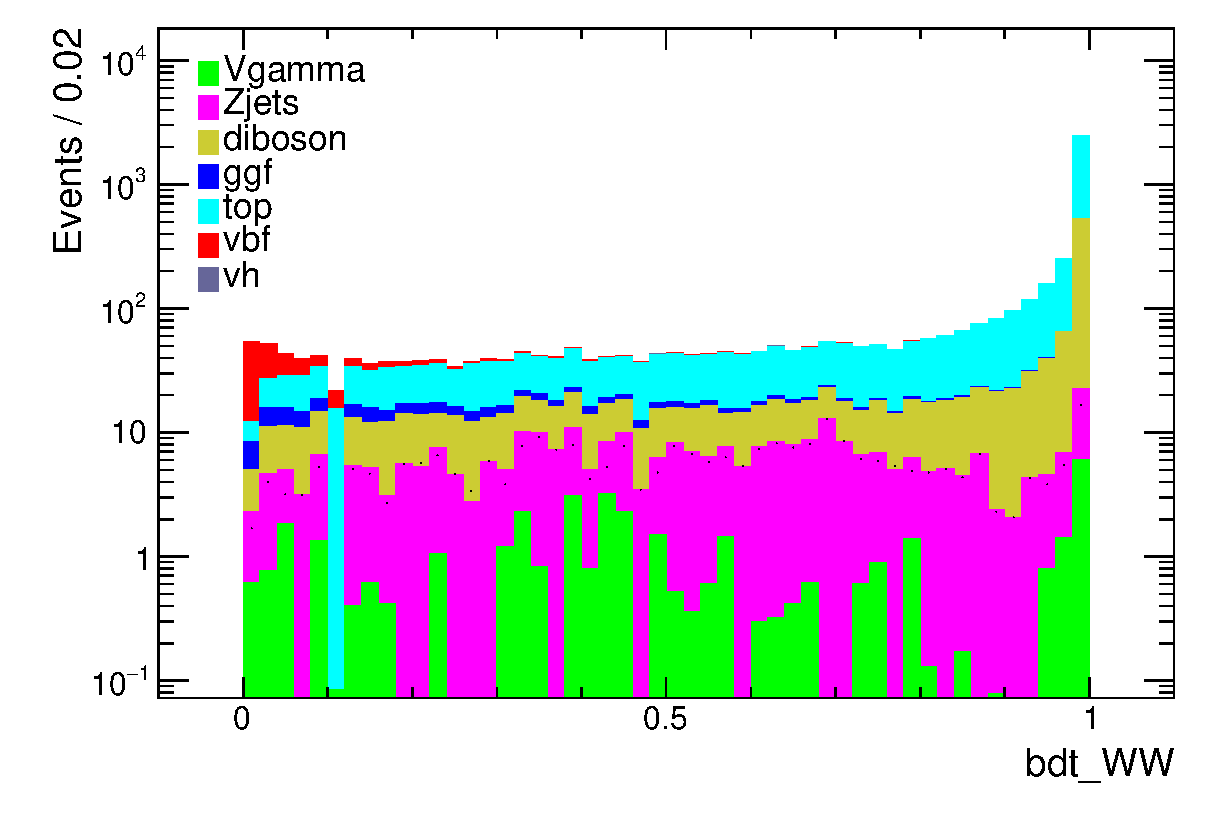
\includegraphics[width=.3\linewidth]{Pictures/finalBDT_def/weightedmulticlassdiboson.eps} 
\caption{Weighted samples of VBF, ggF, and WW as well as all other background samples plotted over BDT output distributions projected onto each axis.}
\label{fig:multiclassBDTresult2}
\end{figure}

A Gaussian quantile transformation is applied to each of the multiclass BDT output distributions. Using the Root function \textit{Cephes::ndtri}, or the inverse of a normal distribution, new distributions spread such that the area under the probability density function from $-\inf$ to each transformed value $x$ is equal to the original value $y$. Using these transformations has led to increased significance over the distributions as shown in Figure~\ref{fig:multiclassBDTresulttrans}.

\begin{figure}[!htbp]
\centering
  \centering
  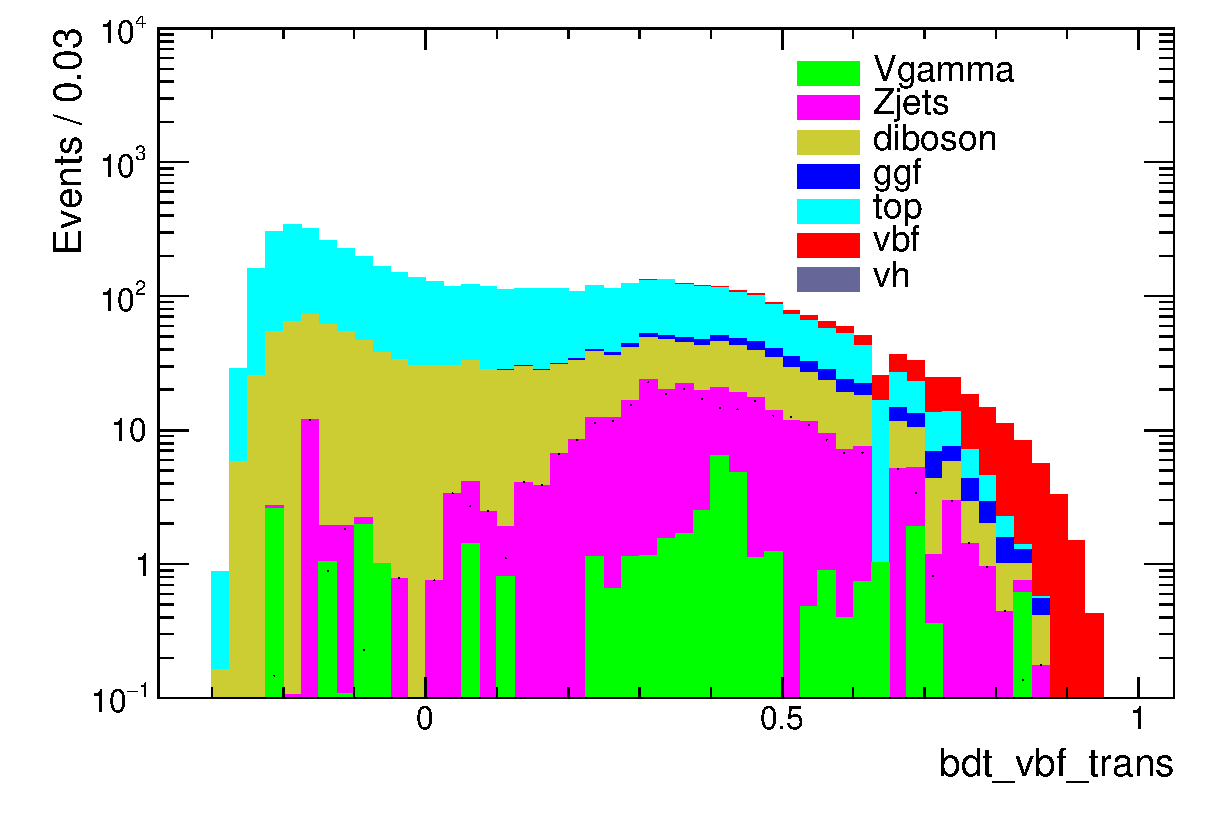
\includegraphics[width=.3\linewidth]{Pictures/finalBDT_def/weightedmulticlassvbftrans.eps} \quad
  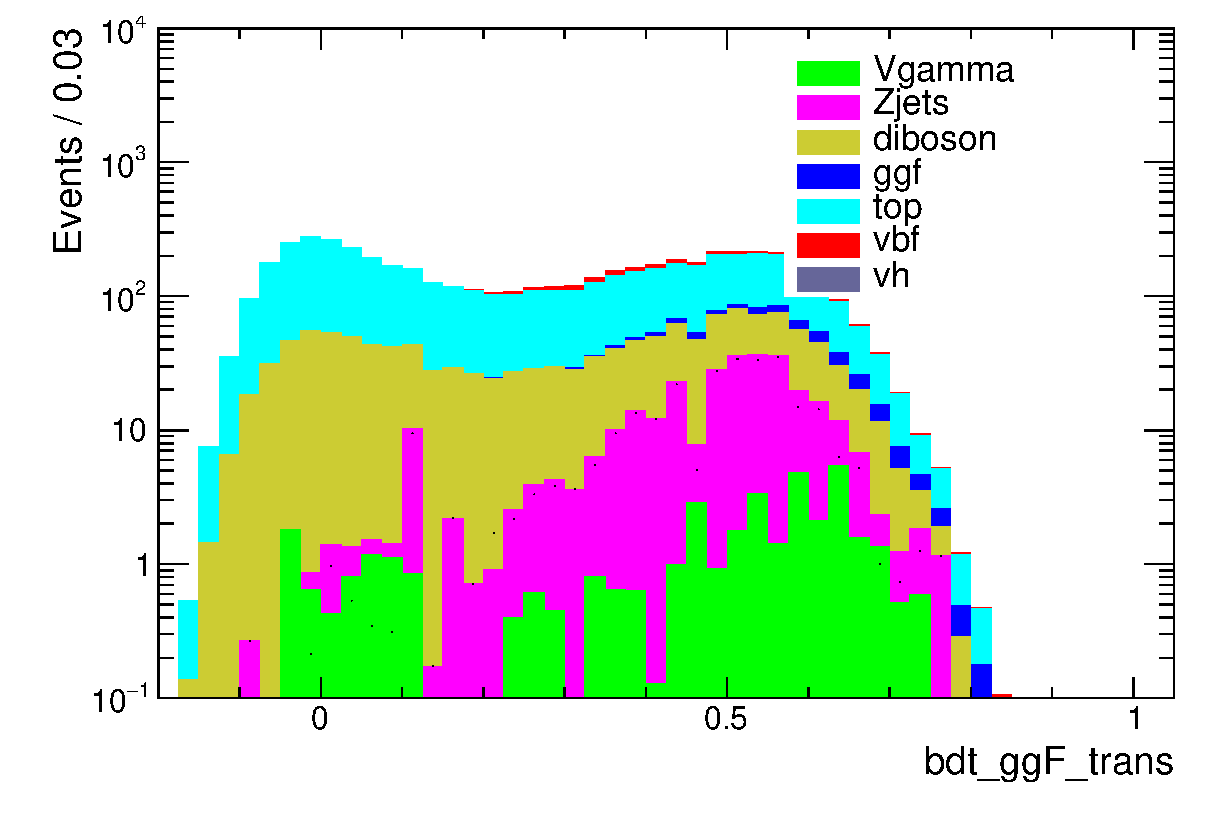
\includegraphics[width=.3\linewidth]{Pictures/finalBDT_def/weightedmulticlassggftrans.eps} \quad
  \includegraphics[width=.3\linewidth]{Pictures/finalBDT_def/weightedmulticlassdibosontrans.eps}
\caption{Weighted samples of VBF, ggF, and WW as well as all other background samples plotted over BDT output distributions transformed with a Gaussian quantile function and projected onto each axis.}
\label{fig:multiclassBDTresulttrans}
\end{figure}

Two key metrics for testing the success of our multiclass BDT are $S/B$ and signal significance examined both bin-by-bin and summed over the entire distribution. Figure~\ref{fig:multiclass3D} shows the distribution of the VBF signal, all combined backgrounds, and signal significance in 3D across all BDT outputs. The signal significance is defined as $S/\sqrt{S+B}$. The overall expected significance can be calculated by adding simple significance bin-by-bin in quadrature to obtain the value of 7.6. For a more accurate value, the following significance definition is summed in quadrature:
\[
    Z = 
\begin{cases}
    +\sqrt{2(n\ln[\frac{n(b+\sigma^2)}{b^2+n\sigma^2}]-\frac{b^2}{\sigma^2}\ln[1+\frac{\sigma^2(n-b)}{b(b+\sigma^2)}])},& \text{if } n\geq b\\
    -\sqrt{2(n\ln[\frac{n(b+\sigma^2)}{b^2+n\sigma^2}]-\frac{b^2}{\sigma^2}\ln[1+\frac{\sigma^2(n-b)}{b(b+\sigma^2)}])},& \text{if } n<b .
\end{cases}
\] 
where $b$ denotes background estimates with a statistical uncertainty $\sigma$ and $Z$ represents significance of seeing $n$ signal events. This definition of signal signicance is the current recommendation from the ATLAS statistics committee~\ref{Buttinger:2643488}. Adding this definition of signal signifiance bin-by-bin quadratically gives an overall value of 10.3.

\begin{figure}[!htbp]
\centering
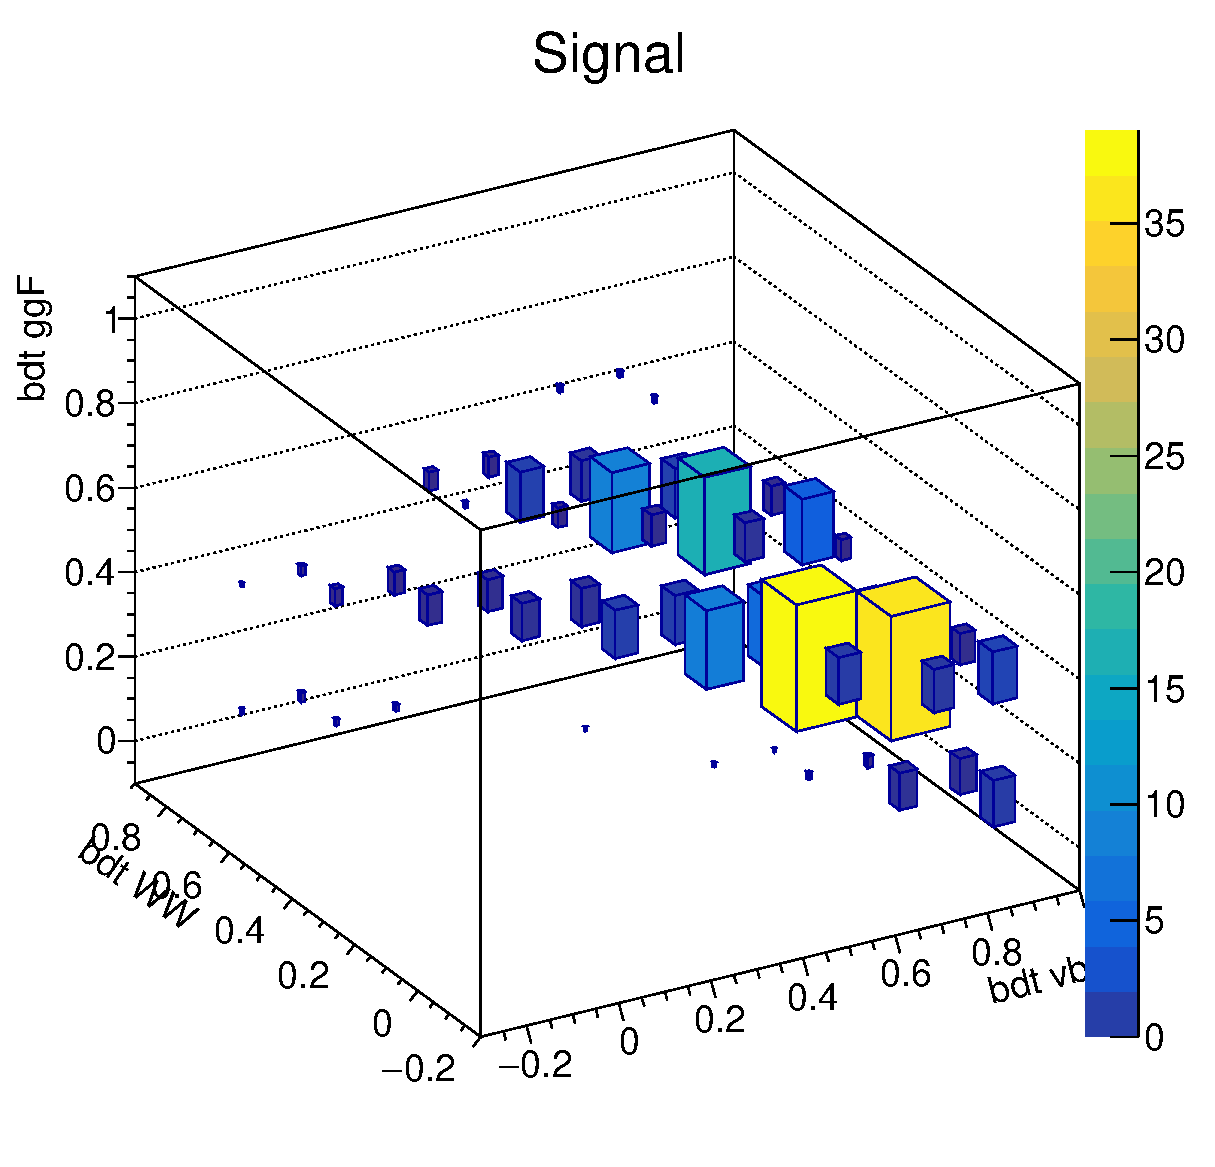
\includegraphics[width=.4\linewidth]{Pictures/finalBDT_def/Signalfull_trans_simp.eps} \quad
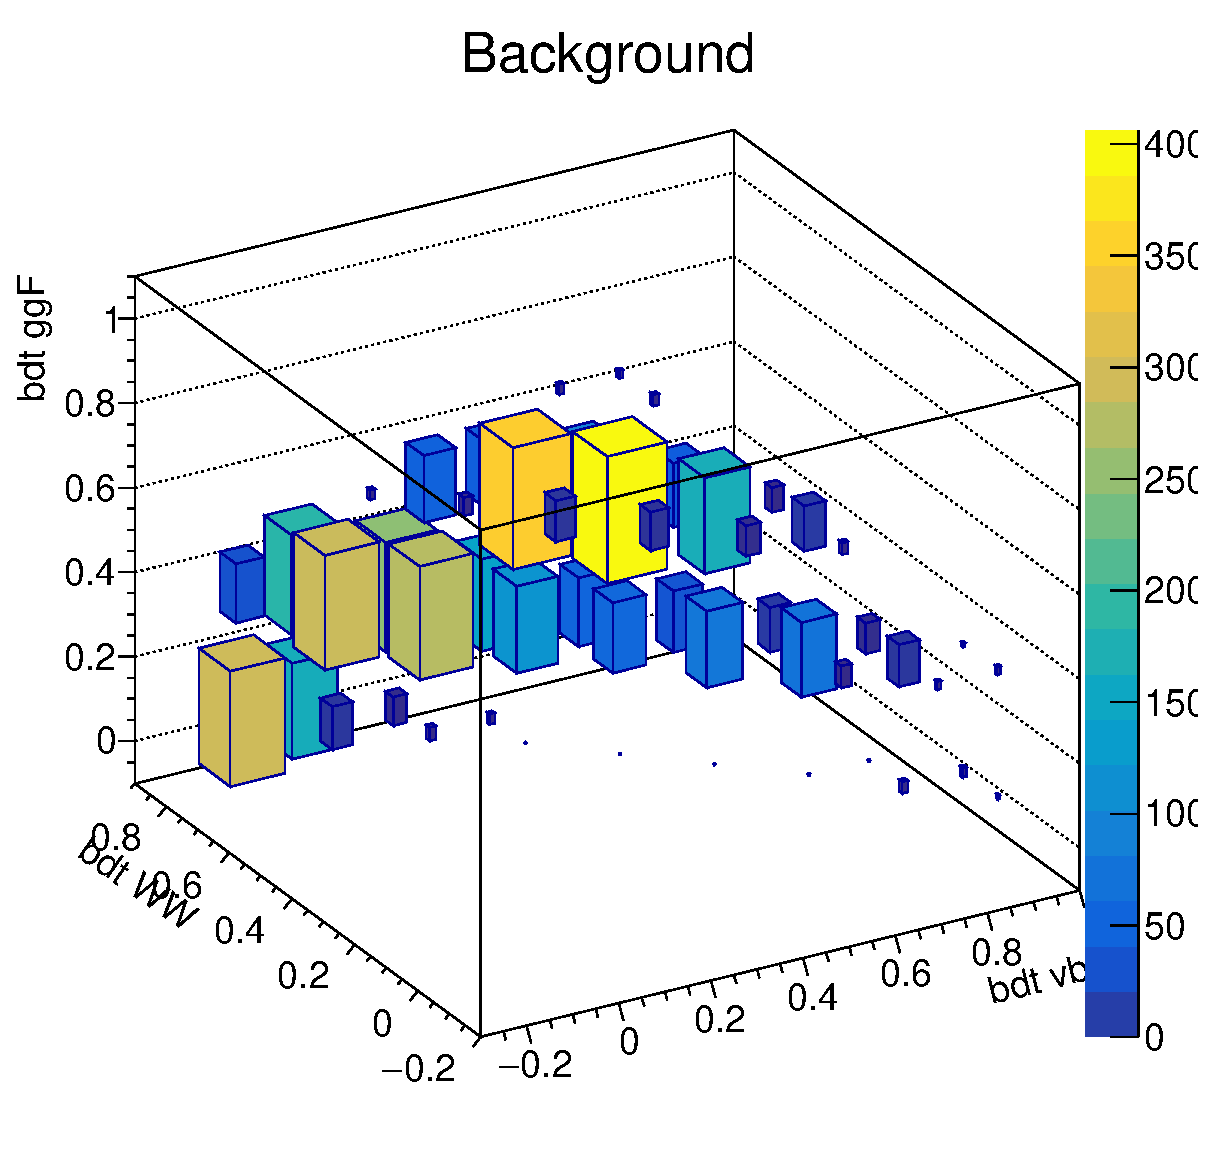
\includegraphics[width=.4\linewidth]{Pictures/finalBDT_def/Backgroundfull_trans_simp.eps}
\medskip
\includegraphics[width=.4\linewidth]{Pictures/finalBDT_def/Significancefull_trans_simp.eps} 
\caption{Plots show 3D distribution of multiclass BDT ouput for VBF signal (top, left), all combined backgrounds (top, right), and bin-by-bin signal significance (lower, center).}
\label{fig:multiclass3D}
\end{figure}

We can similarly calculate simple significance and $Z$ using three 1D BDTs trained and used in the current analysis. While these are trained independently and so do not take into account correlations between BDT outputs, the overall discrimination is greater. These BDTs are detailed in the main text and consist of: VBF vs. ggF, VBF vs. top$+WW$, and top$+WW$ vs. all samples. These do not correspond directly to the 3D BDT (and are combined in the final analysis with additional discrimants for ggF) but can clearly show high discrimination in Figure~\ref{fig:1Das3D} without the need for additional transformations. The simple significance combined in quadrature is $8.9$ and the $Z$ is calculated at $10.1$. These are very similar to the values shown from the 3D BDT training and combined with the ABCD method employed to further reduce ggF background, provide better overall discrimination.

\begin{figure}[!htbp]
\centering
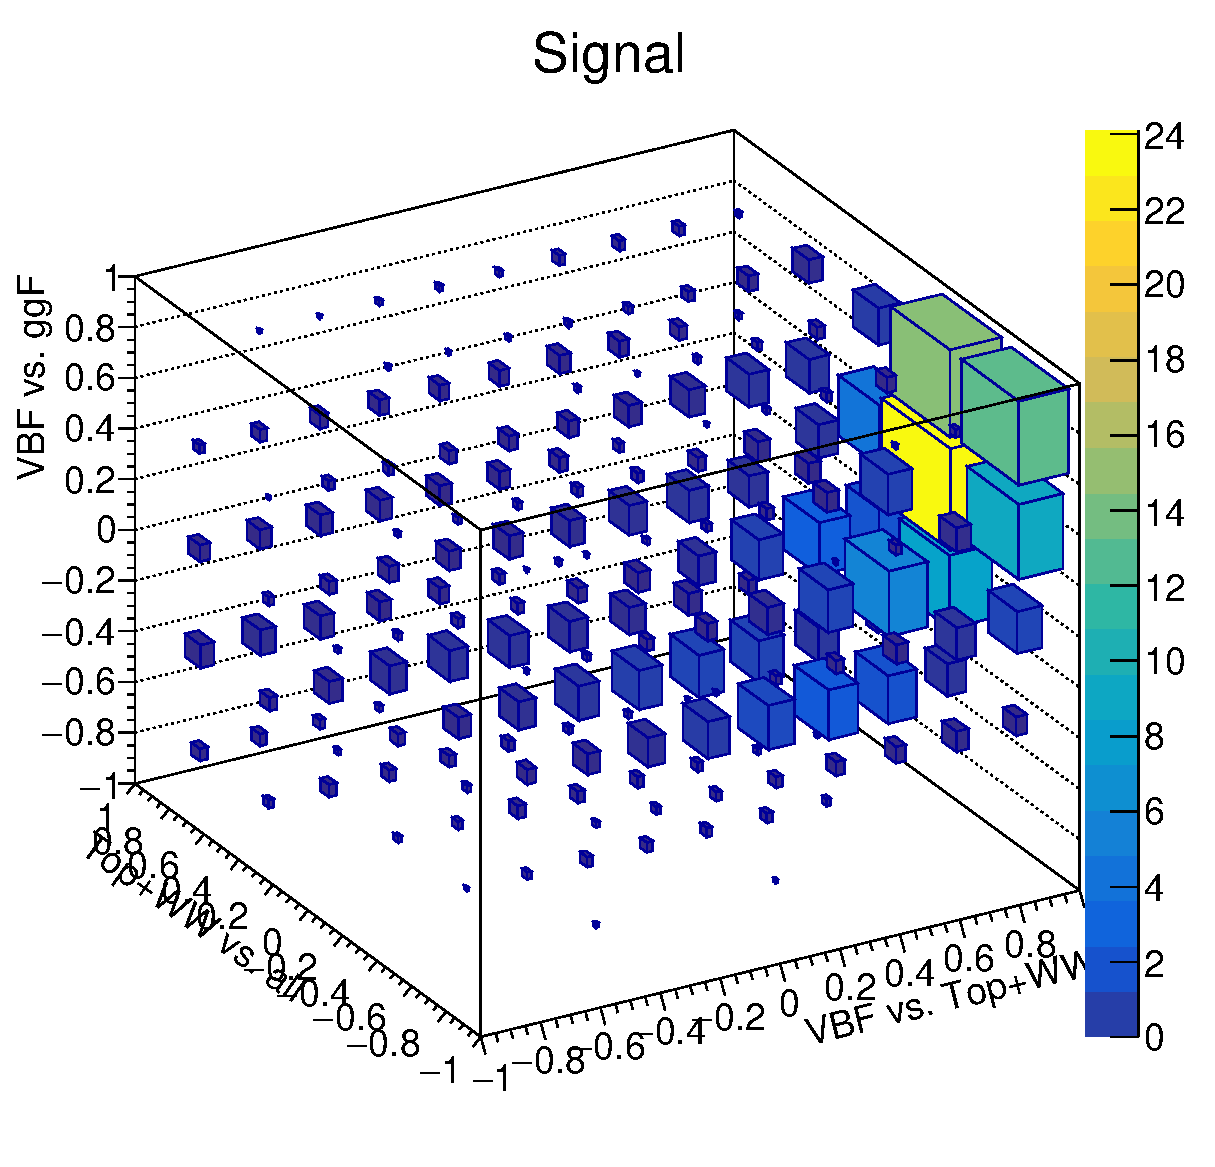
\includegraphics[width=.4\linewidth]{Pictures/finalBDT_def/Signalfull_1D_simp.eps} \quad
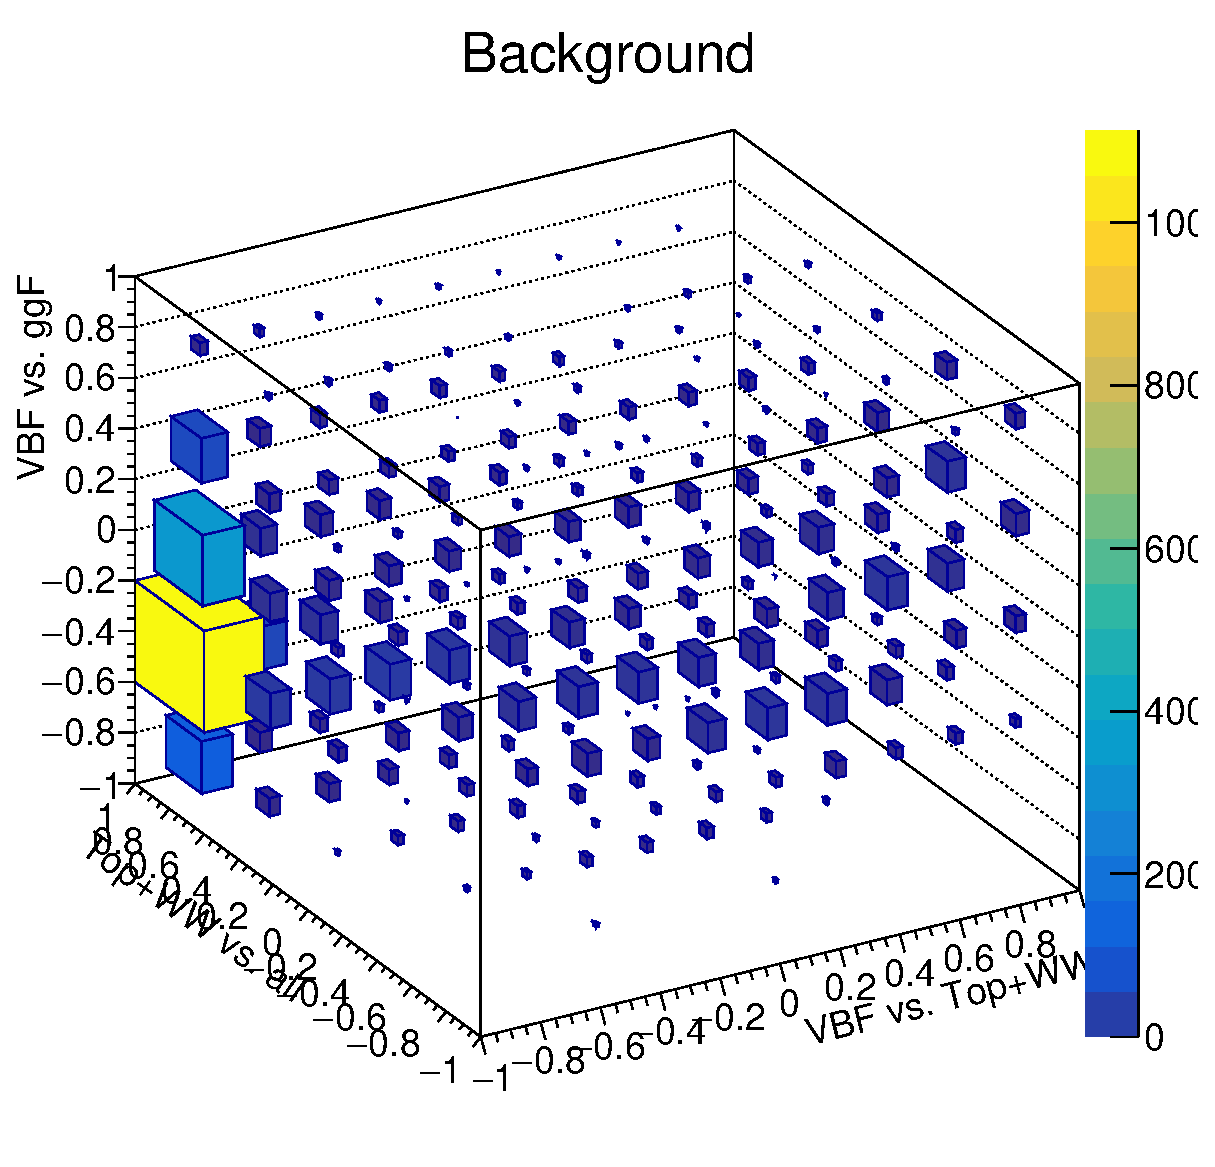
\includegraphics[width=.4\linewidth]{Pictures/finalBDT_def/Backgroundfull_1D_simp.eps}
\medskip
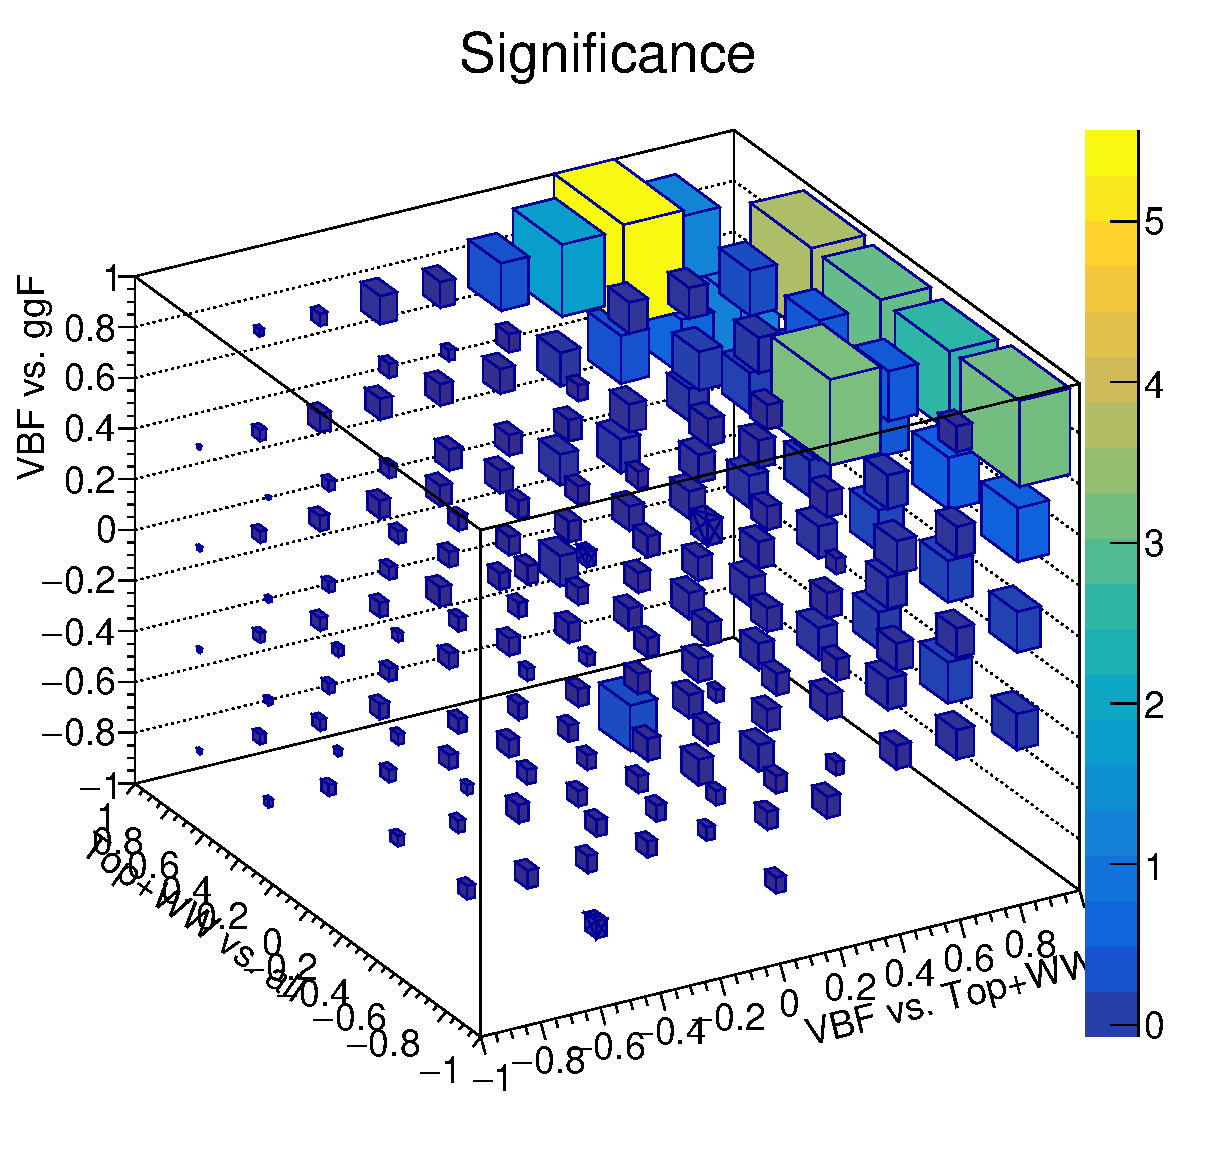
\includegraphics[width=.4\linewidth]{Pictures/finalBDT_def/Significancefull_1D_simp.eps} \quad
\caption{Plots show 3D distribution of 1D BDT ouputs for VBF signal (top, left), all combined MC background (top, right), and bin-by-bin signal significance (lower, center).}
\label{fig:1Das3D}
\end{figure}

Both methods leave out additional contributions from fake and $ttH$ backgrounds and both use the same cuts on the $\Ztt$ BDT for best comparison, though this cut is not used in the final method. The binning in both cases is slightly different to optimize discrimination in each case. 

